\documentclass[11pt]{article}
\usepackage{graphicx}
\usepackage{caption}
\usepackage{subcaption}
\usepackage{geometry}
\usepackage{url}
\geometry{
  a4paper,
  total={170mm,257mm},
  left=20mm,
  top=20mm,
}

\author{David Burian}
\title{YouTube Sound Classification}

\newcommand{\Log}[1]{{\small\texttt{#1}}}
\newcommand{\Fn}[1]{{\small\textit{#1}}}
\newcommand{\File}[1]{{\small\textsf{#1}}}

\begin{document}
\maketitle

\section{My approach}

I was fairly new to audio-processing tasks, and so the first thing that I did
was to read up on topics regarding to sound-processing. This included the
following topics:
\begin{itemize}
  \item Fast Fourier Transform, Discrete Fourier
    Transform, and Discrete Cosine Transform,
  \item Spectograms, log-spectograms, Mel-spectograms,
  \item Cepstograms, Mel-cepstograms,
  \item various other features of sounds like Root Mean Square Energy or Zero
    Crossing rate,
  \item just few models such as Wav2vec, Hubert, Whisper, which are probably
    getting pretty old, but I wanted to
    have rough idea about the architectures used,
  \item I refreshed my knowledge of CTC loss.
\end{itemize}

Even though I didn't end up needing all of the knowledge I gathered, it was fun to
learn and explore. After the study session I planed to approach the task as so:

\begin{enumerate}

  \item Look at the data, and understand them and the type of task.
    (Section \ref{section:data_analysis})

  \item Try easy solutions to the problem. Apply off-the-shelf models from
    scikit-learn and see what you'll learn. (Section \ref{section:sklearn_baselines})

  \item Train a neural network to get the best score possible. (Section \ref{section:nn_models})

\end{enumerate}

\section{Data Analysis}\label{section:data_analysis}

\begin{itemize}
  \item[] \textbf{Relevant notebooks:}
    \begin{itemize}
      \item \File{data\_analysis.nb.py} -- for Sections \ref{section:getting_to_know_data} and \ref{section:splitting}
      \item \File{feature\_engineering.nb.py} -- for Section \ref{section:train_data}
    \end{itemize}
\end{itemize}

\subsection{Getting to know the data}\label{section:getting_to_know_data}

As with all other ML projects, I knew that proper data analysis is crucial and
I spent good amount of time by looking at the data. First I listened to few
examples per label combination. I identified the samples by index in the
\texttt{tsv} files. These were my findings:


\begin{itemize}
  \item not a cleanly annotated dataset
  \begin{itemize}
    \item labels don't include everything that happens
    \begin{itemize}
        \item e.g.
        \begin{itemize}
            \item `133` missing instrument,
            \item `681` missing wind,
            \item `78` missing speech,
            \item `124` missing vehicle, music,
            \item `753` and `931` missing speech
            \item `328` missing speech
        \end{itemize}
    \end{itemize}
    \item labels sometimes stand for events that take up minority of the recording
    \begin{itemize}
        \item e.g.
        \begin{itemize}
            \item `643` 1s taken up by true label music,instrument, 9s unlabelled speech
            \item `931` 8s of unlabelled talking, 2s of labelled tool
            \item its not like events happen in the middle of the recording -- sometimes they are at the beginning, sometimes at the end
        \end{itemize}
    \end{itemize}
  \end{itemize}

  \item few mislabellings (extras and errors)
  \begin{itemize}
    \item e.g.
    \begin{itemize}
        \item `191` extra animal
        \item `623` extra animal
        \item `231` baby noise is sometimes interpreted as animal
        \item `1523` extra vehicle
        \item `1899` rap being recognized as signing
    \end{itemize}
  \end{itemize}

  \item speech includes multiple languages
  \item multi-labels are order-invariant
  \begin{itemize}
    \item sometimes its impossible to say which comes first
    \item sometimes they happen at the same time
    \item if they are in order, the order doesn't need to correspond to the label order
    \item for some combination more than one order exists in the dataset
    \begin{itemize}
        \item e.g.
        \begin{itemize}
          \item `'Music,Musical instrument'` and `'Music,Musical instrument'`
          \item `'Speech', 'Animal'` and `'Animal', 'Speech'`
        \end{itemize}
    \end{itemize}
  \end{itemize}

  \item singing sometimes means just concert noise
  \item there is a 'silence' label
  \item not all clips are 10s
  \begin{itemize}
    \item e.g.
    \begin{itemize}
        \item `706` 8s
        \item `930` 9s
    \end{itemize}
  \end{itemize}

  \item volume of clips is not the same
  \begin{itemize}
    \item e.g.
    \begin{itemize}
        \item `954` a lot quieter than `1304`, (same labels)
    \end{itemize}
  \end{itemize}

  \item duplicates
  \begin{itemize}
    \item e.g.
    \begin{itemize}
        \item `3290` ('Animal', 'Speech', 'Music') and `139` ('Speech', 'Music')
        \item `7020` ('Music', 'Musical instrument', 'Speech') and (I know I heard it already, I just couldn't find the previous file)
        \item `3` ('Water',) and `111` ('Water',)
    \end{itemize}
  \end{itemize}

  \item distorted audio
  \begin{itemize}
    \item e.g.: `9753`
  \end{itemize}
\end{itemize}

To summarize:
\begin{itemize}

  \item the dataset is not cleanly annotated: labels are missing or (rarely) are extra

  \item there are duplicates in the dataset

  \item labelling is order invariant, meaning the task is not to predict the
    \emph{sequence} of labels, just their \emph{presence}

  \item there are some technical gotchas to watch out for:
    \begin{itemize}
      \item 'Silence' label exists, meaning we cannot cut-out audio with low volume
      \item volume differs, which suggests that I should consider using some kind of normalization
      \item not all clips are 10s, but almost all of them are at max 10s long
    \end{itemize}

  \item the labelling distribution is heavily biased, with some combinations
    appear only once per dataset

\end{itemize}

\subsection{Creating train and dev split}\label{section:splitting}

After getting the 'feel' for the data, I wanted to split them up to train and
development split. This would allow me to analyse the train data more in
detail, without worrying about overfitting. I decided against using separate
'test' split, because it would decrease the amount of data for training and I
wouldn't be able to make further decisions after seeing an evaluation on the
test split (since then it would be just another validation split).

\subsubsection{Trying to get rid of duplicates}

However, before splitting I wanted to take some time to resolve the duplicate
audios. Duplicates are bad since they cause information leakage in between
splits and they might help with the annotation cleanliness. I started by
looking at the duplicate audios I found and compared their signal as in Figure
\ref{fig:duplicates}.

\begin{figure}
  \centering
  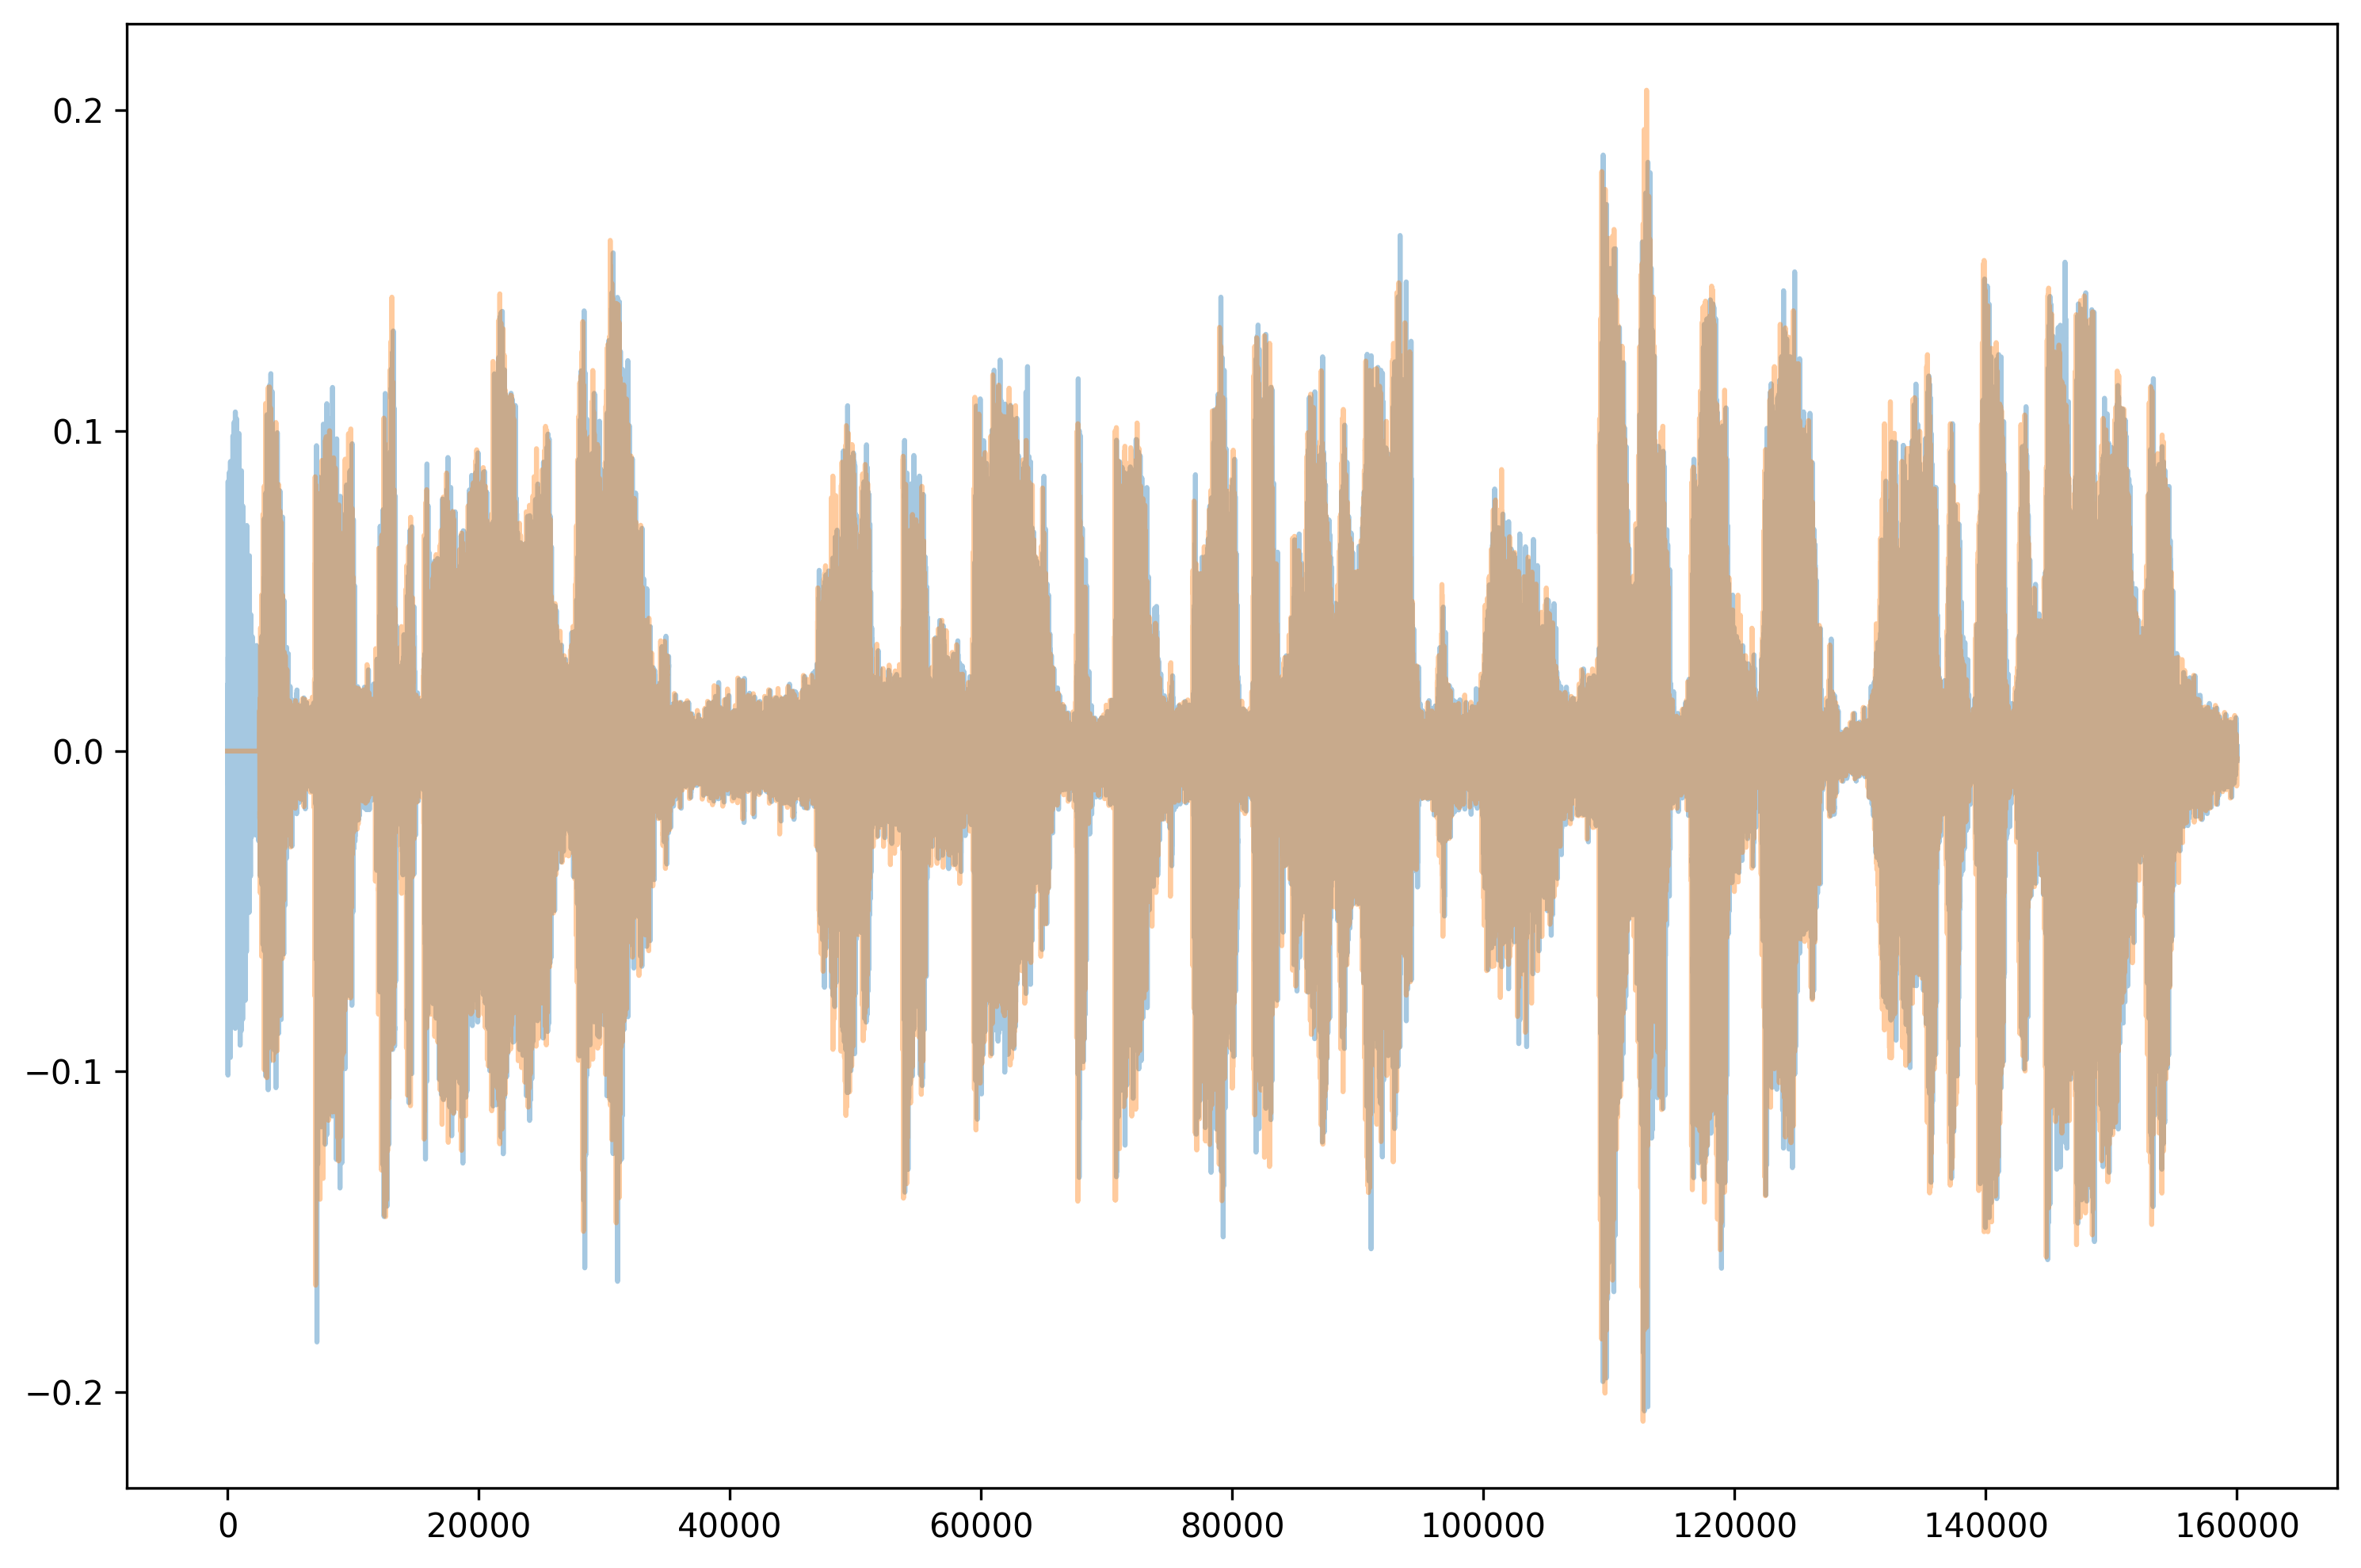
\includegraphics[width=0.8\textwidth]{../notebooks/imgs/duplicate_audio_example.png}

  \caption{Duplicate signals with ids `3290` and `139`. `139` is shifted by
  2550 samples forward.}\label{fig:duplicates}

\end{figure}

I tried several approaches to identify the duplicate signals:

\begin{enumerate}

  \item Naively trying to find shift of one signal such that the difference
    between the two signals would be minimal.

  \item Using off-the-shelf fingerprinting library

  \item Applying K-NN to chunks of MFCCs with large windows.

\end{enumerate}

The first approach surprisingly yield large differences even for almost
completely overlapping signals. This meant that the decision boundary between
``It's a duplicate'' and ``It's not a duplicate'' was fairly small. So small I
didn't want to rely on in. For the second approach I tried to use
DejaVu\footnote{\url{https://github.com/tuxdna/dejavu}}, but the PyPi package
was outdated, installation cumbersome and the project seemed abandoned. So I
settled for \texttt{ctoth}'s
repo\footnote{\url{https://github.com/ctoth/audioprint}}. However it failed to
recognize even the duplicates that I found, so I got rid of it. The last
solution chunked-up MFCCs and fed them to a KNN model. During retrieval, I got
audios whose chunks were on average closest to the queried chunks. This worked
surprisingly well. I found that a distance below 100, is almost always a
duplicate. On the other hand, the smallest distance to non-duplicates, from
what I have seen, was around 150. After seeing around 50 query results, I got
pretty confident that this technique might be able to successfully identify at
least a portion of duplicates. However, I wasn't totally sold and decided to
postpone further de-duplication experiments.

\subsubsection{Actually splitting data to train and dev split}

I split the data in 80:20 ratio, according to the distribution of labels, so
that both splits reflect the same data distribution. Note, that I didn't split
the data according to the samples' label combinations, but rather according to
a label's presence. In case one audio got to be in both splits, I removed it
from the training split. My reasoning was that, we'd want the detection of
different sounds to be independent. So we split the data as if they were
independent (even though it might be harder to detect speech during a heavy
metal concert).

In the end, I don't think this mattered as much since both distributions -- of
labels and of label combinations -- ended up being very similar, as can be seen
in Figure \ref{fig:label_distributions}. 80:20 ratio gave me around 2k audio
samples to validate on, which I think is plenty.

\begin{figure}

  \centering
  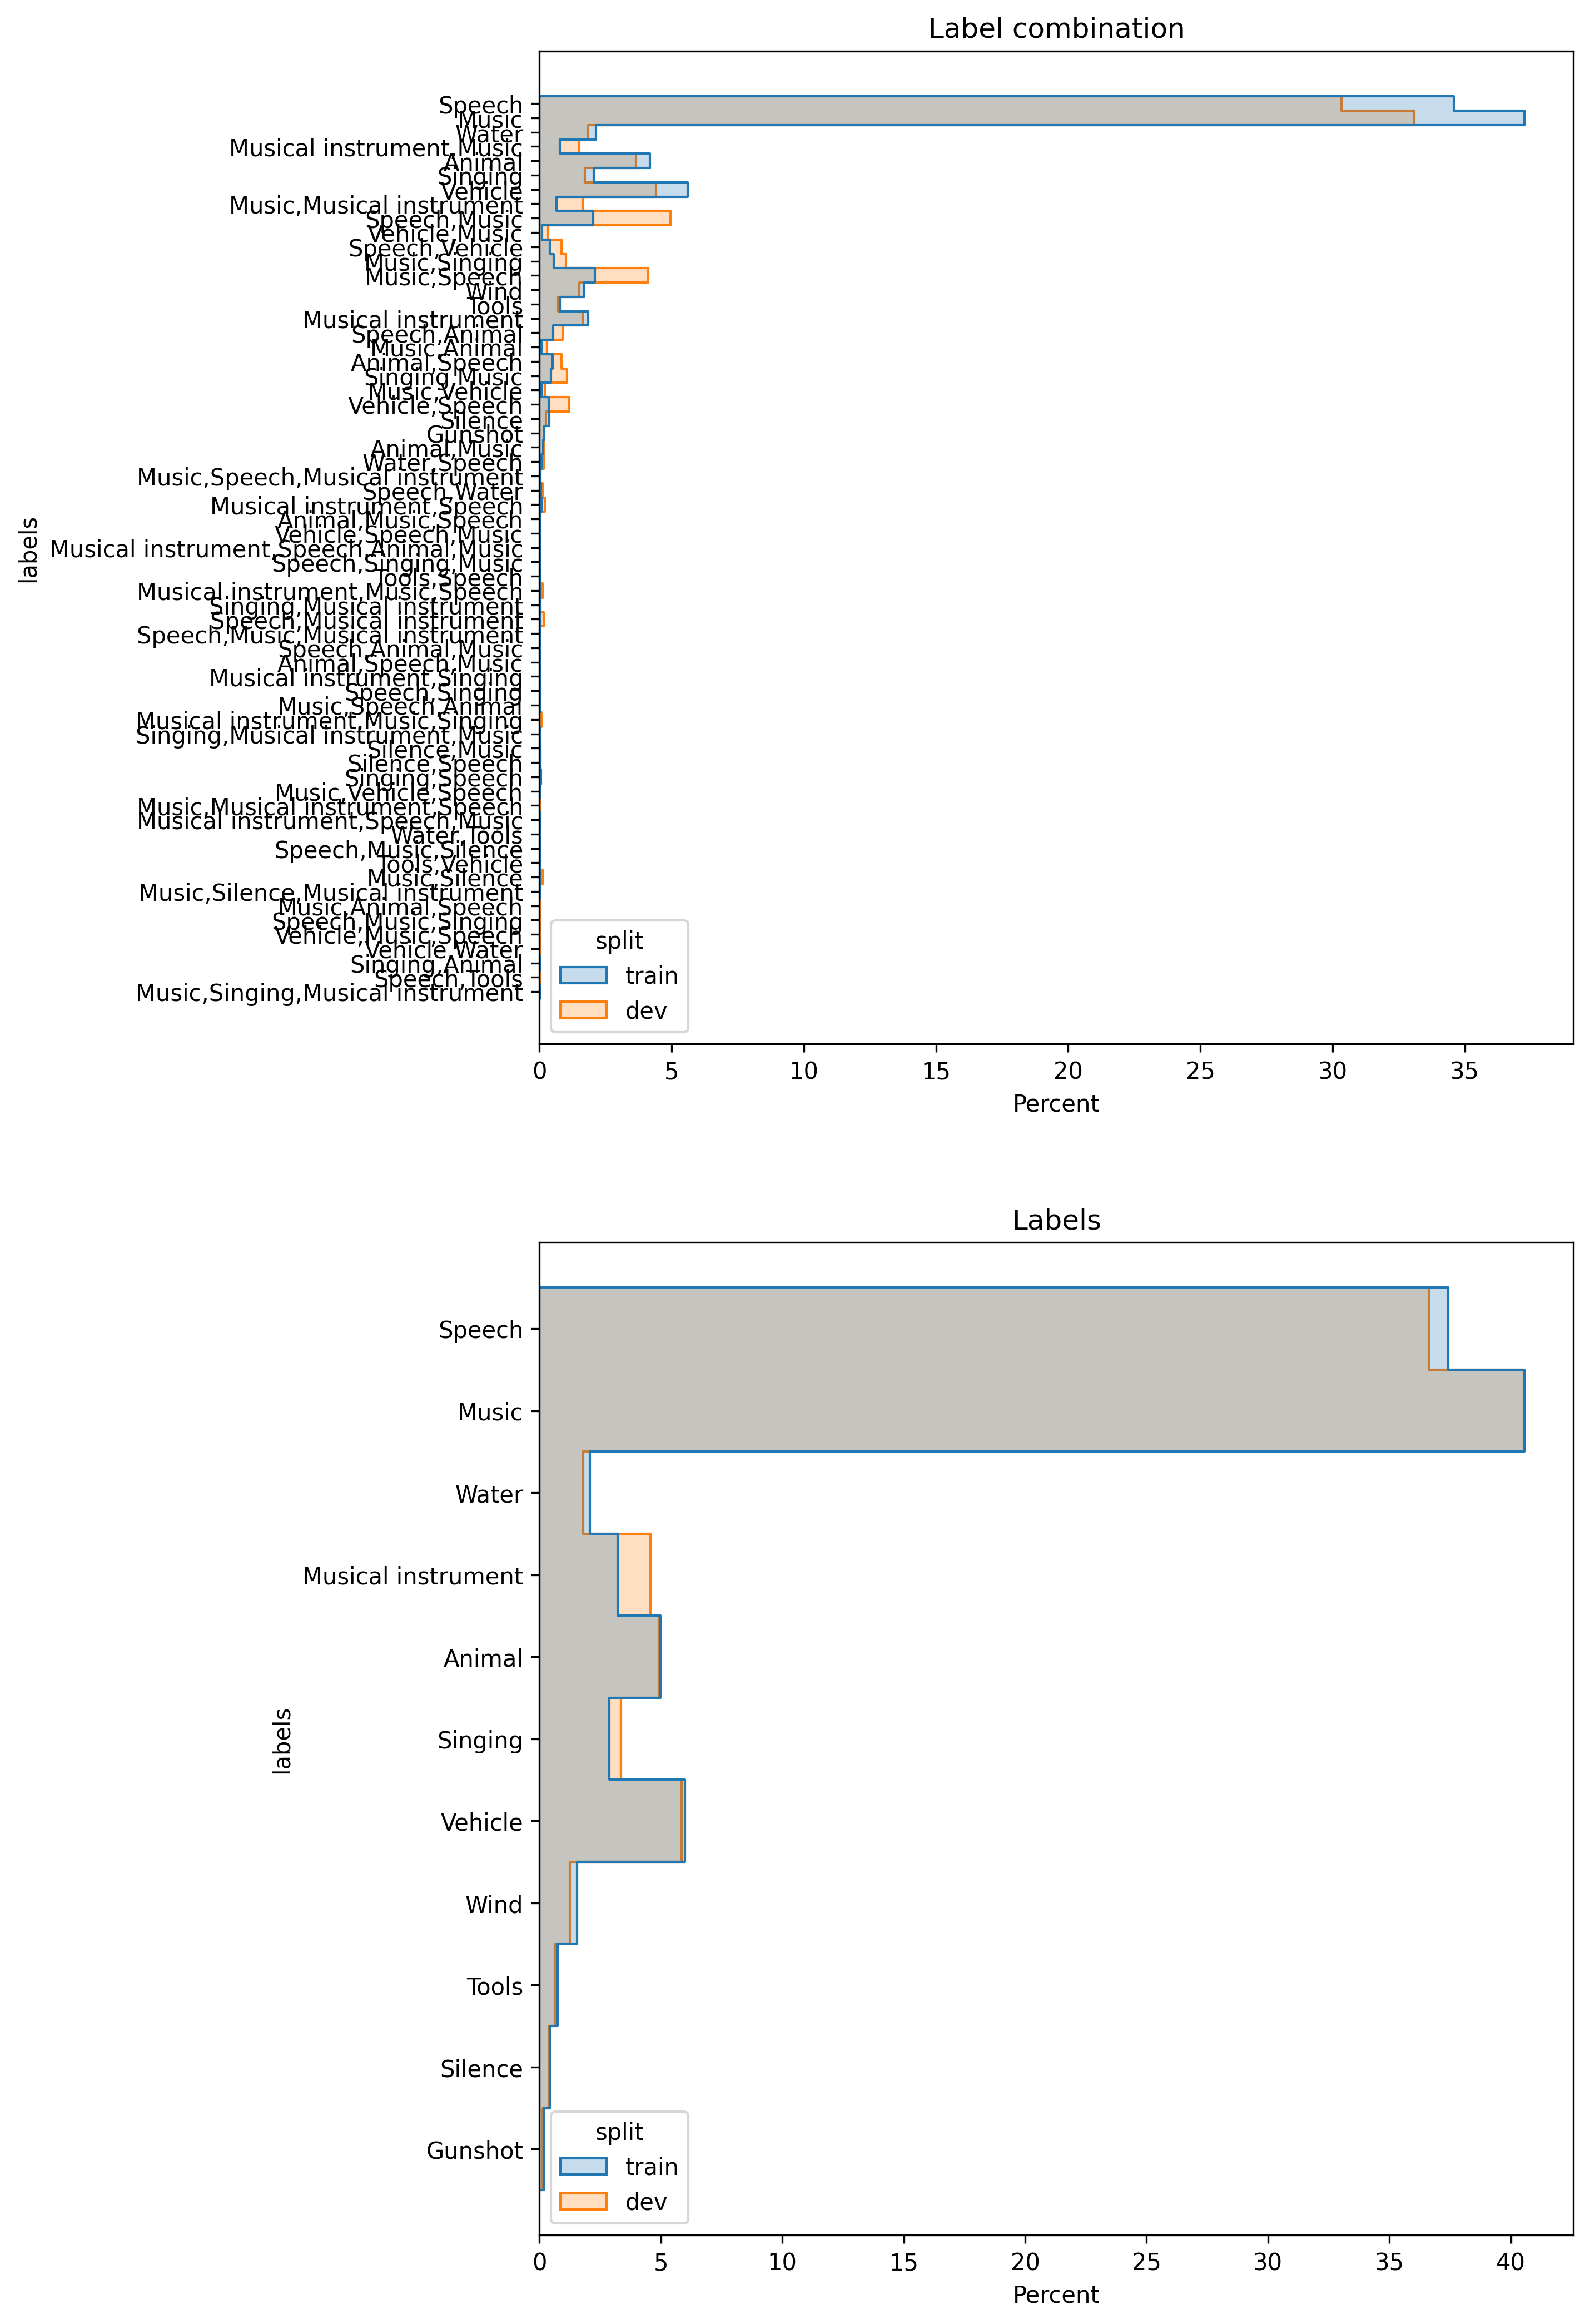
\includegraphics[width=0.9\textwidth]{../notebooks/imgs/dev_train_distributions.png}

  \caption{Comparison of label distributions for train and dev splits. Notice
  that dev split has more label combinations, a bit less of speech and a bit
  more of musical instruments.}\label{fig:label_distributions}

\end{figure}

\subsection{Closer look at training data}\label{section:train_data}

I took a second look at the train data to see the best features. I looked at
loudness, RMS, ZCR. All of which are plotted in Figure \ref{figure:features}. Due to
the label combinations, a lot of the distributions (per label) are similar.
However, there are some exceptions:

\begin{itemize}
  \item `Silence''s RMS is quite separable from the other labels
  \item `Water''s and `Tools''s ZCRs are also quite separable from the other labels
\end{itemize}

The two distinctions above could be used to construct an informed classifier.
However, as the separation is not great, I decided to postpone this idea, but
in the end I didn't have time to come back to it.

\begin{figure}
    \centering

    \begin{subfigure}{\textwidth}
      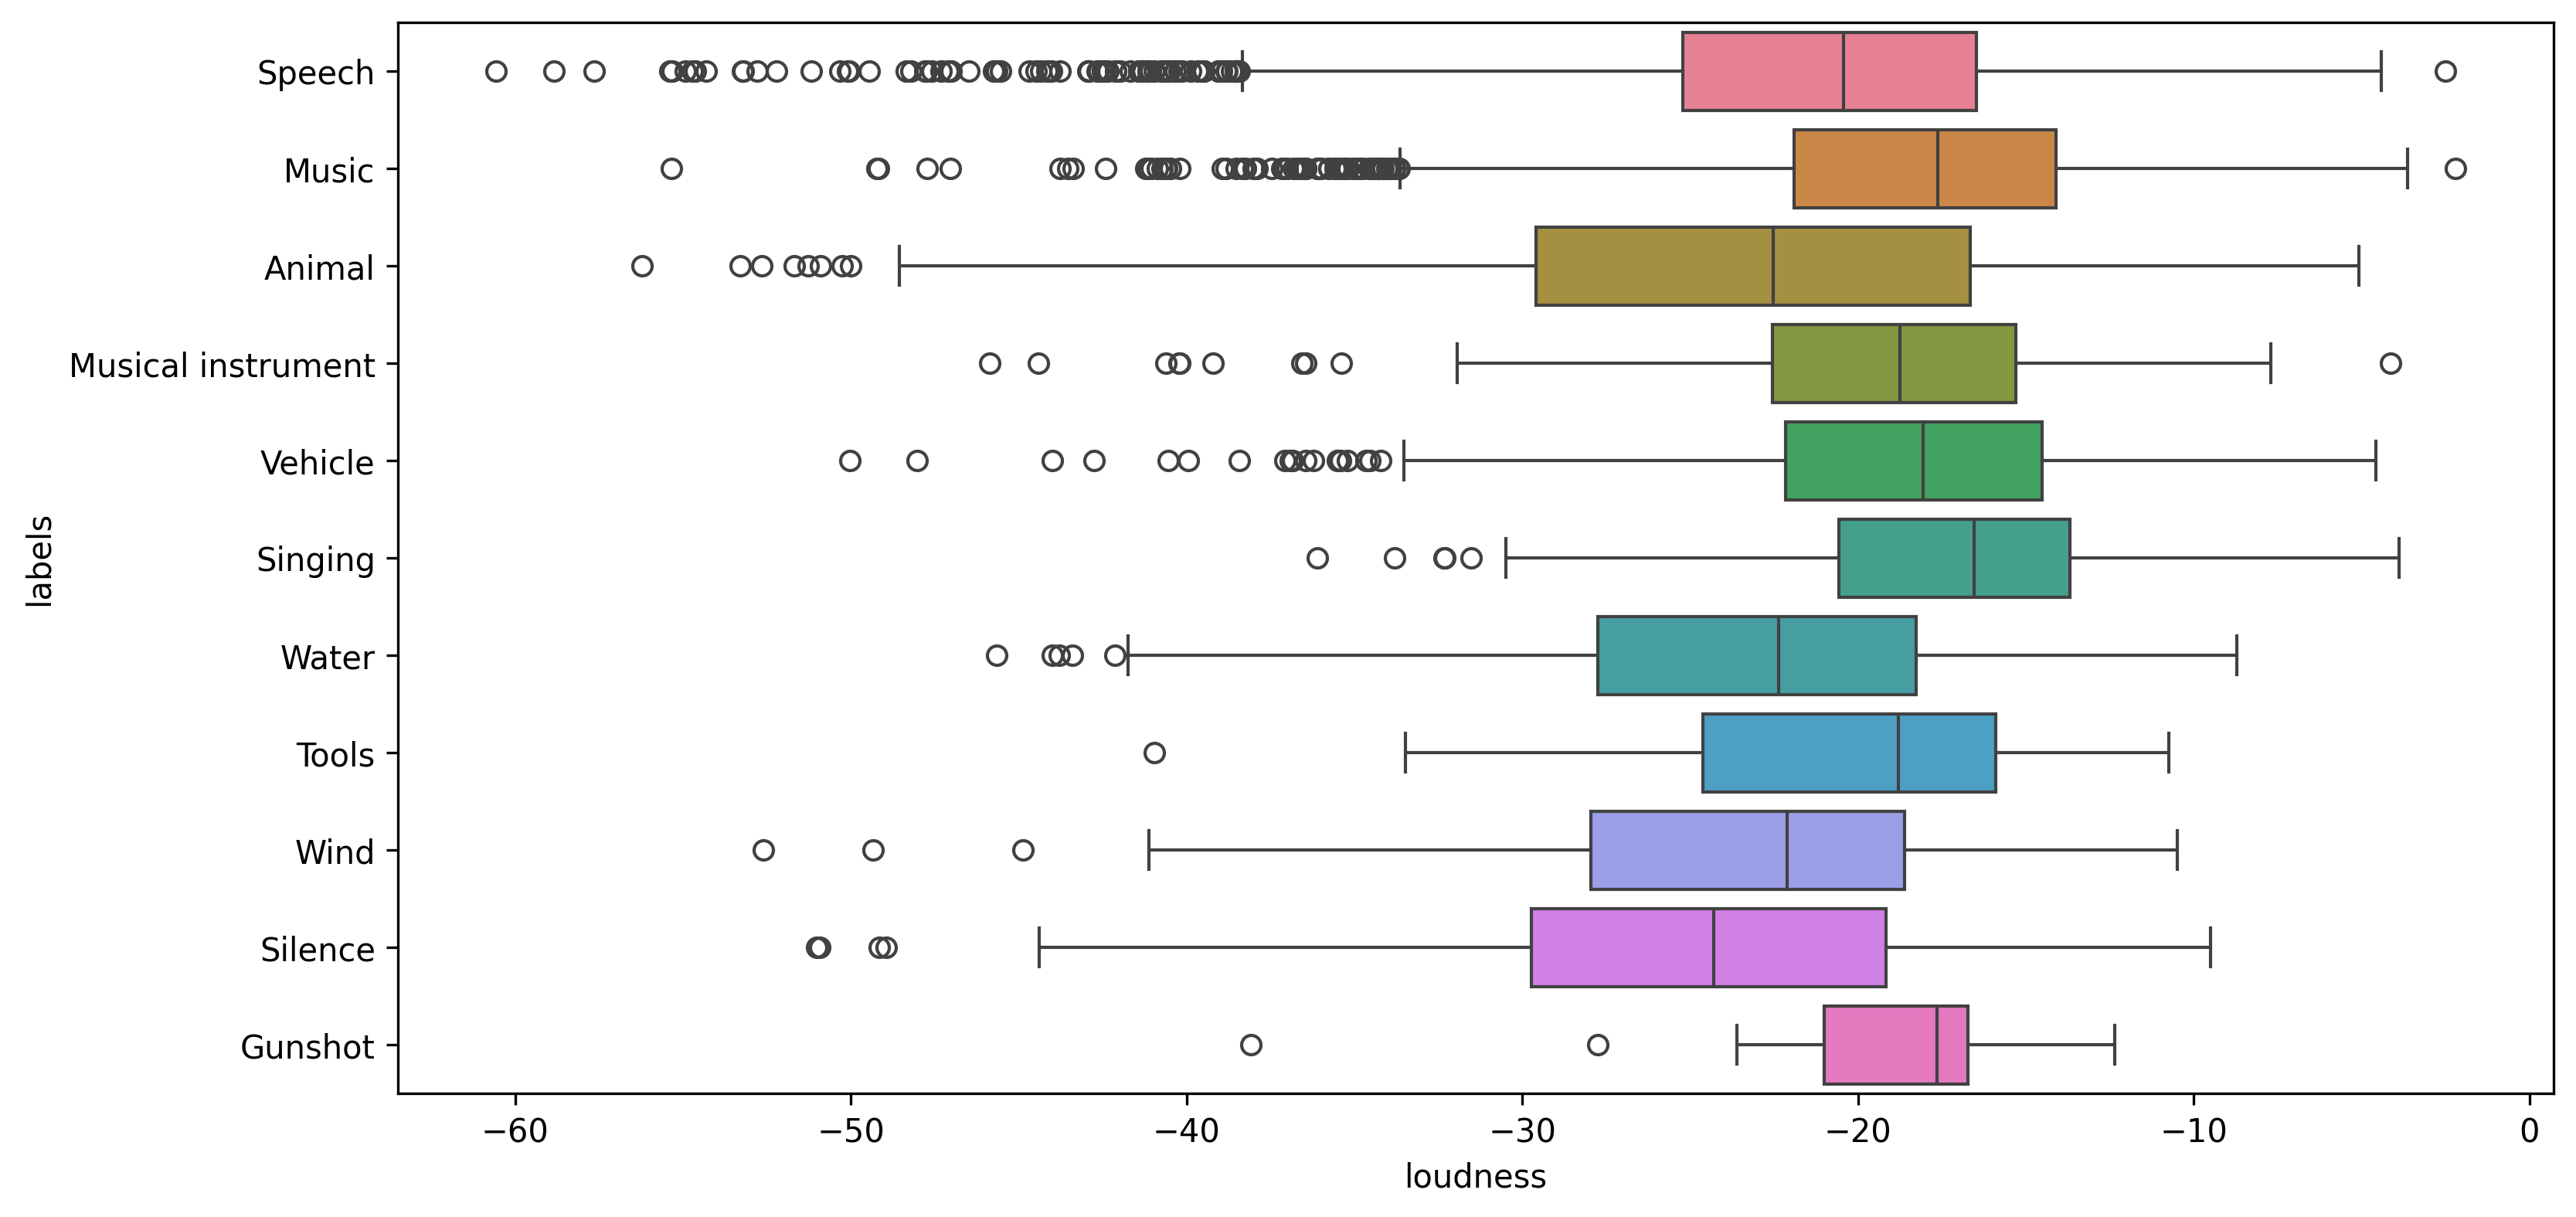
\includegraphics[height=0.3\textheight]{../notebooks/imgs/loud_dist.png}
    \end{subfigure}
    \begin{subfigure}{\textwidth}
      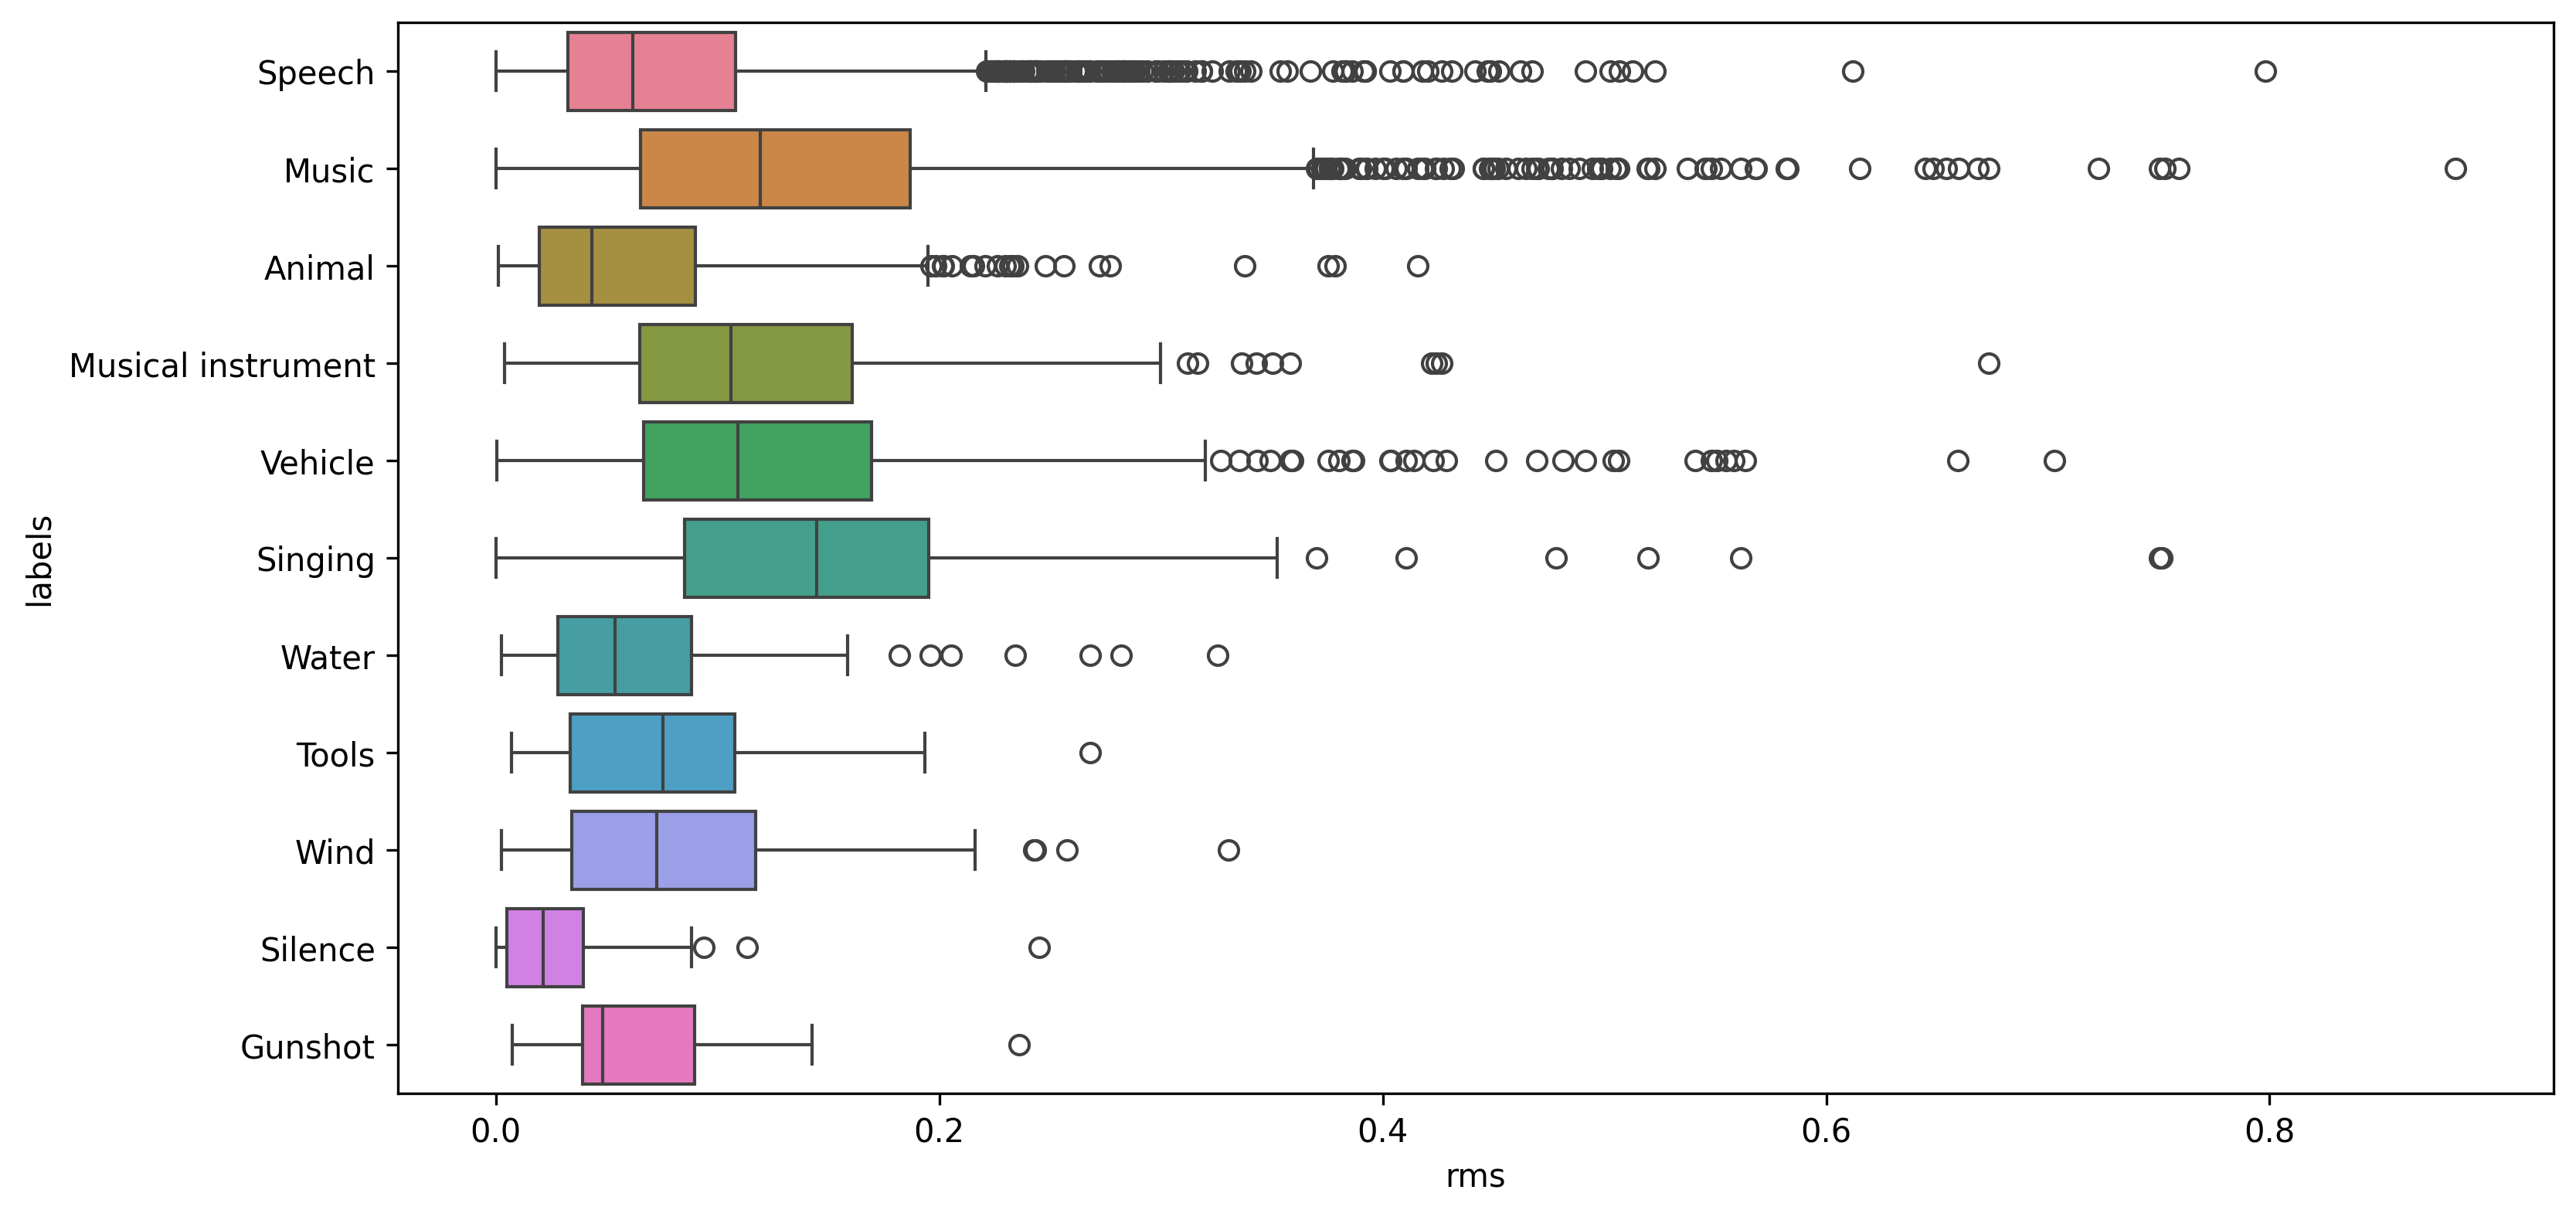
\includegraphics[height=0.3\textheight]{../notebooks/imgs/rms_dist.png}
    \end{subfigure}
    \begin{subfigure}{\textwidth}
      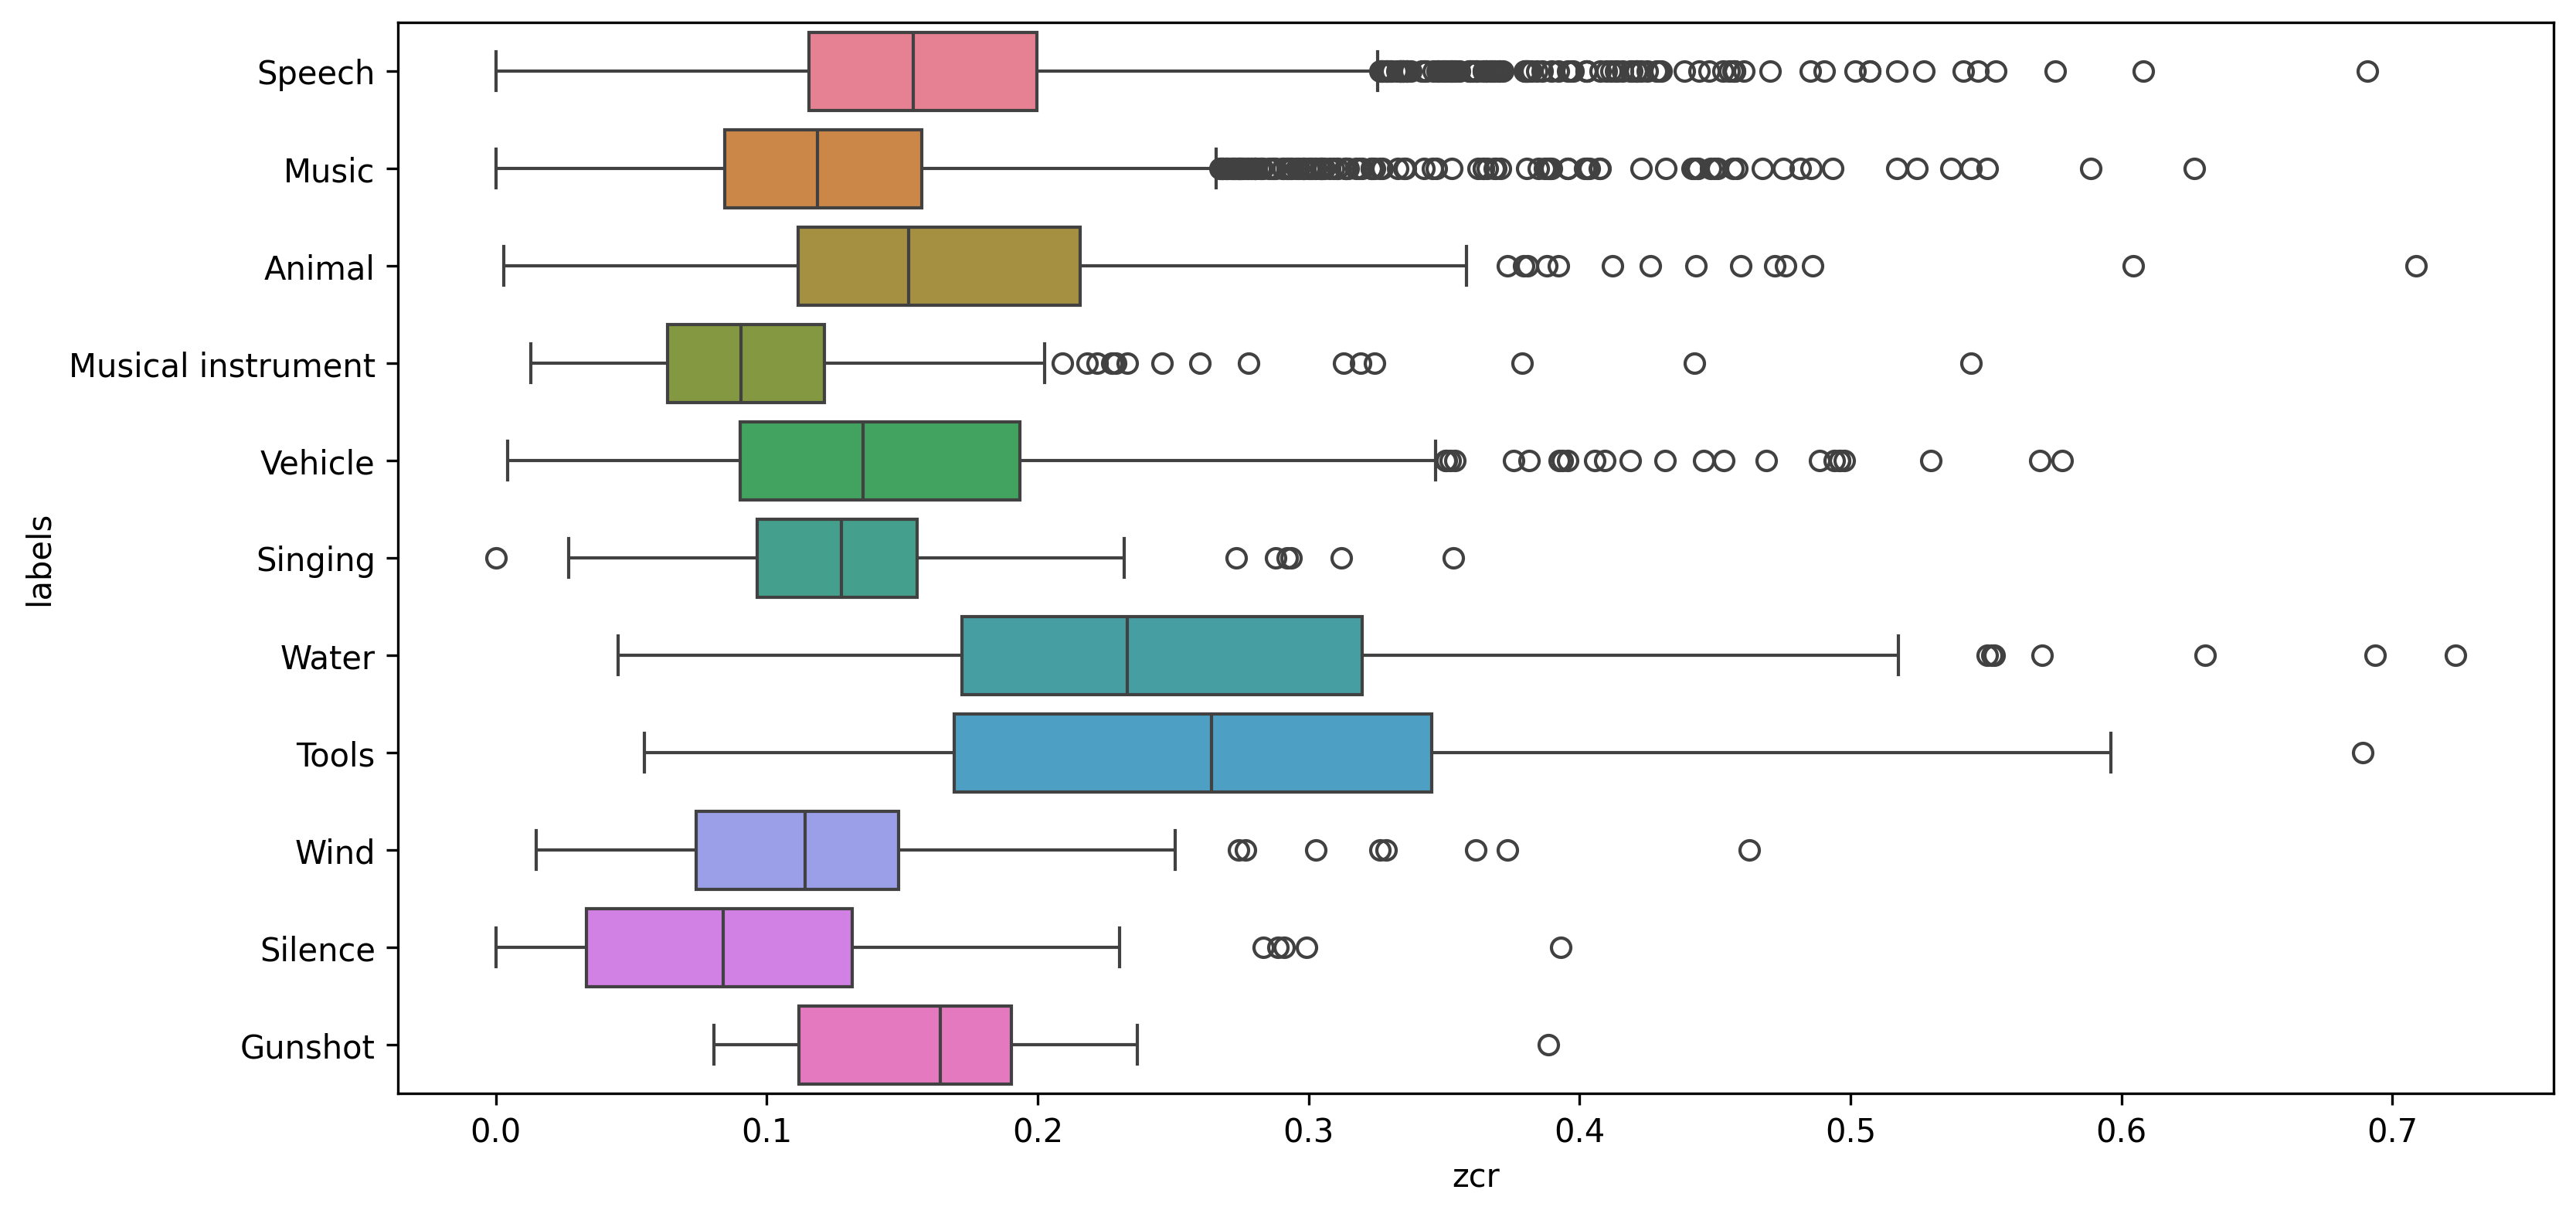
\includegraphics[height=0.3\textheight]{../notebooks/imgs/zcr_dist.png}
    \end{subfigure}

    \caption{Distribution of Loudness, Root-Mean-Square energy, and Zero
    Crossing rate of signals in training split.}\label{figure:features}

\end{figure}

\subsubsection{Frequency filtering}

I also wanted to see if there are some high or low frequencies, which I could
filter out without risking filtering out any major features. However, after
playing with amplitude thresholds, I discovered the signals span the entire
spectrum from 0Hz to 8000 Hz. I could have filtered out some 30Hz on the bottom
end, but I don't think that would have mattered.

\subsubsection{Projecting MFCCs to 2d}

This experiment was a bit arbitrary, but I wanted to see if PCA + TSNE could
uncover some structure in the space of MFCCs. This was largely inspired by my
de-duplication k-NN model, that worked better than expected. I applied PCA to
get cover 0.9 variance, and projected these components to 2d using TSNE.
However, the projection is a 2d 'blob', which doesn't really tell us anything.

\begin{figure}
  \centering
  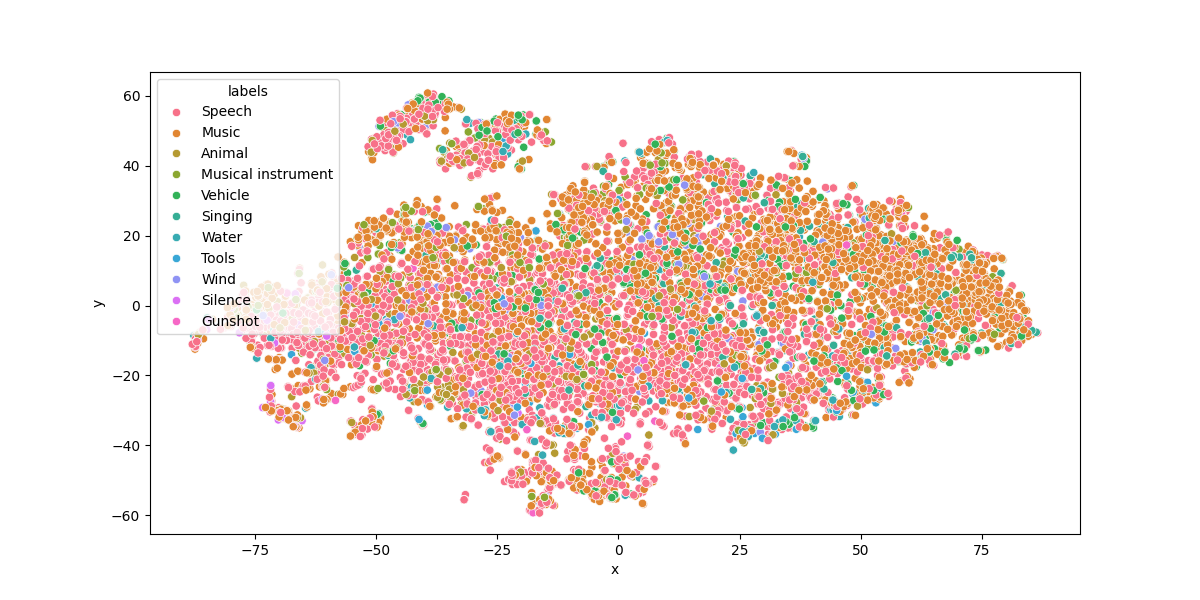
\includegraphics[width=0.9\textwidth]{../notebooks/imgs/pca_mfccs.png}

  \caption{Projection of MFCCs to 2d using PCA to 51 components, than TSNE to 2.}
\end{figure}

\subsection{Looking at MFCCs}

Since I wasn't very familiar with MFCCs I wanted to get the 'feeling' for them,
similarly as I did with the audio clips. I wasn't sure if MFCCs are better
features than just Mel spectrograms, but in the end I experimented almost only
with MFCCs. I think, here some extra familiarity with sound processing would
pay off. I wasn't sure if the information encoded in the MFCCs is visible
enough, and if it isn't, how to highlight it.

\subsection{Visualizing transformations}

Later, during training of neural networks I experimented with several
augmentations. To debug and test the augmentations, I used the rest of the
notebook \File{feature\_engineering.nb.py}.

\section{Experiments}

\subsection{Metrics}

Throughout my experiments I kept an eye on precision, recall, f1 and support. I
chose the main metric to be macro-averaged f1-score. This simulates a scenario
where we want to achieve good performance on all labels and we value TP and TN
equally.

\subsection{Scikit-learn solutions}\label{section:sklearn_baselines}

\begin{itemize}
  \item[] \textbf{Relevant notebooks:}
    \begin{itemize}
      \item \File{sklearn\_baseline.nb.py} -- experimenting with sklearn models
        (not runnable)
    \end{itemize}
\end{itemize}

I tried 3 sklearn models to fit on MFCCs: K-NN, Random Forest (RF) and SVM. The
motivation for these experiments was the successful de-duplication model which
was based on similarity of MFCCs of different signals. For all 3 models I
repeated the following 3 steps:

\begin{enumerate}
  \item Overfit on train split
  \item CrossValidate on train split to get the best hyperparameters
  \item Evaluate the best variant on dev split
\end{enumerate}

All 3 models easily overfitted, however, showed very poor performance on
validation split. The performance was so poor, I stopped experimenting with
these models and moved on. Later the codebase changed a bit, and so, the
notebook currently \emph{cannot be run}, as it relies on interface that
no-longer exists.

\subsection{Neural network models}\label{section:nn_models}

\begin{itemize}
  \item[] \textbf{Relevant notebooks:}
    \begin{itemize}
      \item \File{training.nb.py} -- running trainings
      \item \File{cnn\_train\_testing.nb.py} -- testing various aspects of training
    \end{itemize}
  \item[] \textbf{Relevant modules:}
    \begin{itemize}
      \item \File{youtube\_asr.train} -- creating \Fn{DataLoader}s and \Fn{Trainer}
      \item \File{youtube\_asr.preprocess} -- data preprocessing functions and augmentation
      \item \File{youtube\_asr.dataset} -- loading dataset
    \end{itemize}
\end{itemize}

For a neural network model I followed the standard procedure: overfit on
training split with smallest model possible, then regularize to improve
validation metrics.

\subsubsection{Overfitting on train split}

I started by generating fairly limited MFCC:
\begin{itemize}
  \item 13 MFC coefficients
  \item 1024 window length
  \item 256 hop length
  \item 64 Mel filters
\end{itemize}

I experimented with several small network architectures before arriving to the following:

\small
\begin{itemize}
  \item 8d, (3, 7) kernel, (1, 5) stride, ReLU
  \item 16d, (3, 5) kernel, (1, 3) stride, ReLU
  \item 4 of ResNet-like small blocks, where each block has:
    \begin{itemize}
      \item 16d, 3 kernel, 1 stride, 0 padding, ReLU
      \item 16d, 3 kernel, 1 stride, 0 padding
      \item sum with residual connection
    \end{itemize}
  \item 4096d, ReLU
  \item 128d, ReLU
  \item 11d
\end{itemize}
\normalsize

I trained with common settings:
\begin{itemize}
  \item Adam optimizer, learning rate $10^{-4}$
  \item Cross-Entropy Loss
  \item batch size 8
\end{itemize}

The above settings were able to overfit on 1 batch in 2.7k steps as seen in log
\Log{whimsical\_lemming/version\_24}.

To describe the following experiments in reasonable amount of space, I will
describe only the experiment's differences compared to the previous experiment.

\begin{enumerate}
  \item \Log{flat\_wrasse/version\_0}: batch size 16, overfitting on 20\% of training split
  \item \Log{grumpy\_squirrel/version\_0}: batch size 32, overfitting on 50\% of training split
  \item \Log{gainful\_vulture/version\_0}: overfitting on 80\% of training split in 50k steps
    \begin{itemize}
      \item batch size 64
      \item 32 MFCCs
      \item Initial convolution has (5, 7) kernel, (3, 5) stride
      \item 6 ResNet-like blocks
    \end{itemize}
  \item \Log{versatile\_bonobo/version\_0}: overfitting on 100\% of training split in 23k steps
    \begin{itemize}
      \item transitioned to ResNet-like pre-activation blocks where ReLUs are
        applied before each convolution
    \end{itemize}
\end{enumerate}

\subsubsection{Regularization}

To improve validation performance I started to apply regularization. Following
the previous setup, these are the experiments I've ran and the changes they
introduced:

\begin{enumerate}
 \setcounter{enumi}{4}
 \item \Log{vague\_angelfish/version\_0}: adding Batch Norm between every ReLU
   and convolution
    \begin{itemize}
      \item didn't dramatically increase \Log{val/f1/macro}
      \item it was harder for the model to overfit on train split
    \end{itemize}
  \item \Log{large\_caracara/version\_0}: adding $10^{-4}$ weight decay for non-bias parameters
    \begin{itemize}
      \item similar effects as BN
    \end{itemize}
  \item \Log{successful\_ammonite/version\_0}: adding \Fn{time\_wrap} augmentation
    \begin{itemize}
      \item 100\% probability of applying \Fn{time\_wrap}
      \item Time-wrap got generated once for entire training, which probably
        made overfitting a bit easier
    \end{itemize}
  \item \Log{friendly\_mastiff/version\_0}: adding \Fn{upsample} augmentation
    \begin{itemize}
      \item 60\% probability of applying \Fn{time\_wrap}
      \item Upsampling to even-out label distributions
      \item validation f1 score of label's with large upsampling factor went up
      \item validation f1 score of label's with smaller upsampling factor went down (as expected)
      \item slower overfitting on train split
    \end{itemize}
  \item \Log{pumpkin\_heron/version\_0}: switching to binary cross-entropy
    \begin{itemize}
      \item I decided to give BCE a try since it much better follows the idea of independent predictions per each label
      \item with BCE, the model overfits much more easily
      \item but validation metrics didn't plummet, which I would've expected
    \end{itemize}
  \item \Log{fluffy\_poodle/version\_0}: adding \Fn{rand\_frequency\_mask} augmentation
    \begin{itemize}
      \item 50\% probability of masking out between 0 and 16 MFCCs for all frames
      \item the model had still no problem overfitting
      \item no major improvement on validation metrics
    \end{itemize}
  \item \Log{affable\_caiman/version\_0} -- more data augmentation
    \begin{itemize}
      \item masking out up to 24 MFCCs with 0.7 probability
      \item masking out up to 80 time frames with 0.7
      \item still overfitting very quickly
      \item validation scores seem to suffer more
    \end{itemize}
  \item \Log{ruby\_pronghron/version\_0} -- dramatically decrease model size
    \begin{itemize}
      \item only 2 pre-activation ResNet-like blocks
      \item only one 256d fully connected layer after convolutions
      \item with decreasing model size, validation metrics decreased noticeably
    \end{itemize}
  \item \Log{fabulous\_bear} -- try normalizing MFCCs before applying augmentations
    \begin{itemize}
      \item dramatically worsened validation scores
    \end{itemize}
\end{enumerate}

\subsection{Results}

I disclose the best results I was able to achieve in Table \ref{table:results}.

\begin{table}

  \centering
  \begin{tabular}{ l c c }
    \hline
    experiment name (log dir) & val micro f1-score & val macro f1-score \\
    \hline
    \Log{versatile\_bonobo} & 0.59 & 0.338 \\
    \Log{successful\_ammonite} & 0.60 & 0.32 \\
    \hline
  \end{tabular}


  \caption{Final results on dev split.}\label{table:results}
\end{table}

\section{Issues I faced \& Unresolved problems}\label{section:issues}

Though the dataset isn't large, the task is not straightforward. From my
experience, these are the major challenges:

\begin{enumerate}

  \item Lack of clean validation split. -- the missing/extra annotations cause
    validation split to be less reliable. I can deal with poor quality of
    annotations in the training split, however, I'd like an evaluation that I
    can trust.

  \item Poor generalization across several models. -- I've tested 4 types of
    models and done over 15 experiments with CNN models. Unfortunately, all
    models exhibit poor generalization. I don't think that I approached the
    task wrongly, but I suspect that I miss a piece of the puzzle.

  \item Unbalanced label distributions. -- With some combinations appearing
    only once in a dataset, it's clear that problems will appear. I solved this
    issue by upsampling examples according to their label percentage in the
    dataset. Along with heavy augmentation, this meant that the model saw
    approximately the same number of each label with slightly different input.

\end{enumerate}

\subsection{Learnings}

Along with the problems above I face several technical issues. I was used to
machines with TBs of memory, hundreds of CPUs and (almost) unlimited storage.
Transitioning to a machine with 16GBs of memory, 100GB of free space and 12
CPUs was a bit of wake-up call to pay more attention to efficient data
processing. HuggingFace datasets just don't cut it anymore.

I also acknowledge that I tried maybe too many ideas, spreading my time across
several branches of work. This resulted in lack of time and a list of ideas
that I haven't had time to go through.

\end{document}
